\chapter{Conclusions and Discussion}

\section{Overall model accuracy disparities between languages}

One trend that plainly jumps out in the data from SIGMORPHON 2018 and 2019 is that some languages are persistently more difficult to model than others. 

In SIGMORPHON 2018 task 1 best achieved scores, the SIGMORPHON 2019 task 1 baseline models, and the SIGMORPHON 2019 best achieved scores, models of Old Irish always have the lowest accuracy rate, never higher than 10\%, typically followed in second or third place by Latin. 

On the other end of the spectrum, the Turkic languages included in the SIGMORPHON data (Azeri, Bashkir, Crimean Tatar, Kazakh, Khakas, Tatar, Turkish, Turkmen, Uzbek) have among the highest-accuracy models. In the SIGMORPHON 2018 task 1 with a low data setting, 6 of 9 featured Turkic languages achieved accuracies above 85\%, and the Turkic languages averaged 80\% accuracy while the overall mean accuracy was 62\%. In SIGMORPHON 2019 task 1, language pairs with a Turkic target language averaged 74\% baseline accuracy while the overall was 49\%, 81\% best accuracy where the average was 65\%. Curiously, the Turkic languages actually had slightly worse models on average in SIGMORPHON 2019 than 2018, while overall, the accuracy of best models for a given language held constant on average. (The reason that the average best score for Turkic languages was 81\% in 2019 compared to 80\% for 2018 is that higher-accuracy Turkic languages happened to be chosen more often as target languages for transfer pairs in 2019. Best model accuracy for individual Turkic languages decreased by an average of 3\% from 2018 to 2019.)

To some degree, these outcomes correspond with probably expected intuitions or general perceptions of the relevant languages. Turkic languages, for instance, are known for straightforward agglutinative morphology and almost entirely lacking declension classes and irregular forms; for a given grammatical meaning, there is typically a single suffix that is applied to all words \parencite{Johanson1998}. 

\subsection{CMU-03}

There are two language pairs that stand out as seeming outliers in the SIGMORPHON 2019 data, in different ways: Bengali $\rightarrow$ Greek and Swahili $\rightarrow$ Quechua. 

In 2018, the University of Zurich team achieved 32\% accuracy in modeling Greek with a low volume data, the best team on that problem. Greek $\rightarrow$ Bengali and Bengali $\rightarrow$ Greek pairs appeared in SIGMORPHON 2019. The Greek $\rightarrow$ Bengali pair scored fairly typically: the best 2019 model was slightly better than the 2019 baselines and slightly worse than the best 2018 low-resource Greek model. But the Bengali $\rightarrow$ Greek scored only 18\% accuracy from the best 2019 baseline model, yet the Carnegie Mellon team was able to achieve 75\% accuracy on that pair, by far the largest difference between a 2019 baseline and best team performance, and the second-highest absolute improvement between 2018 and 2019. The case of Swahili $\rightarrow$ Quechua is even more drastic: while the best 2019 baseline could only score 14\% accuracy, the same Carnegie Mellon model achieved 92\% accuracy, the single largest disparity between a 2019 baseline and best score.

That model, denoted \texttt{CMU-03} in \cite{McCarthy2019}, had the highest overall accuracy of all submitted models, and was the best performer on 61 of the 100 language pairs, but in particular performed comparatively well on pairs that had done poorly in 2018 or with the 2019 baseline models. \cite{McCarthy2019} et. al. also note that the success of \texttt{CMU-03} is correlated with linguistic similarity of the two languages, though these examples in particular do not provide evidence for that idea. Bengali $\rightarrow$ Greek is a quite distantly related pair, with the two languages belonging to different primary branches of the large and diverse Indo-European family, and Swahili $\rightarrow$ Quechua are completely unrelated. Bengali $\rightarrow$ Greek has fairly typical part of speech distribution overlap and nominal and verbal category overlap, while Swahili $\rightarrow$ Quechua scores substantially below average on all three similarity metrics.

\texttt{CMU-03} is unique in that it employs techniques to attend over morphological tags before ingesting the input lemma, and to bias toward character copying. The effect of these techniques is not clear, but provides an interesting area of future research. Unfortunately, there is no separately published paper or codebase for \texttt{CMU-03}.

\section{Overall outlook for transfer learning as a morphology learning strategy}

\cite{McCarthy2019} states that "gains from cross-lingual training were generally modest, with gains positively correlating with the linguistic similarity of the two languages." The claim that using transferred knowledge boosts model performance, if slightly, seems to come from individual reports from teams about their models. Unfortunately, code or full results for the individual 2019 SIGMORPHON task 1 submissions were not published, so to verify the claim, a comparison of models that differ only in their use of transfer knowledge must be conducted. According to comparison of 2018 and 2019 best models, however, average model performance with or without access to transfer learning was essentially the same, while best model performance varied widely between different pairs.

Given the similarity of data and goals between SIGMORPHON 2018 and 2019, it may be surprising that, for 50 of the 100 training pairs, higher accuracy was achieved on the target language in low-resource settings by the best model of 2018 than by any submission in 2019. It might have been expected that with access to additional data, as well as information from the previous year about which models were successful, models in 2019 should have avoided declining performance. The reason for the performance declines may be that in 2018, the models that performed best in low-resource settings were actually quite different than those that scored well in high-resource settings. Models adapted to low-resource settings tended to avoid pure reliance on neural encoder-decoder models and used techniques such as using string transduction to learn edit sequences and string alignments, and biasing toward copying characters. With the task refocused on neural transfer learning in 2019, many of these techniques might have been dropped. Since all team performances on SIGMORPHON 2019 task 1 were not published, it is not possible to assess the impact of particular model parameters on performance with different types of languages. 

It also may be the case that, since training sets were resampled from 2018 to 2019, the languages that saw worsened performance in 2019 simply had by random chance less useful training sets that year. The low-resource training sets in 2018 and 2019 were relatively small with at most 100 examples, making for greater likelihood of chance sampling effects.

As shown in section 5, from comparison of 2018 and 2019 data, it is far from clear that genealogical relationship between languages leads to effective transfer learning, while verbal category overlap does seem to be significantly predictive of better transfer learning. The statistically significant negative relationship between part of speech distribution similarity and model performance, as well as the suggestive but not statistically significant negative relationship between genealogical closeness and model performance, suggests that transfer knowledge may actually be capable of \textit{confusing} a model. 

% \section{The relationship between category overlap and transfer learning success}


% \section{The relationship between POS distribution similarity and transfer learning success}

\section{Potential language pair sampling confounds}

\subsection{Language pair sampling}

Language pairs for SIGMORPHON 2019 were not selected at random from an even distribution. Many languages appear only as target languages because they lack high-volume data, and some of the languages from the SIGMORPHON 2018 data appear in as many as 5 pairs while others were not included. Some groups of languages, such as Germanic and Turkic groups, appear to have been near-exhaustively paired between a subset of source and a subset of target languages, while the number of fully unrelated pairs is just 7. Genealogical relationship between a language pair appears to be a substantial confound - many results appear statistically significant among non-closely related languages, while no statistically significant inferences could be drawn about the entire pool of language pairs.

\subsection{Turkic languages}

Particular language families also differ from one another, both in internal diversity and in typological trends. In particular, the Turkic family stood out as an outlier in the SIGMORPHON 2019 data. As noted in 6.1, Turkic languages share a set of morphological characteristics that make them relatively easy to model accurately, as evidenced by the higher-than-average accuracy of models over the Turkic languages. The Turkic language family may also be an instance of a family with less internal diversity than, say, the Indo-European family. 

\begin{figure}[ht]
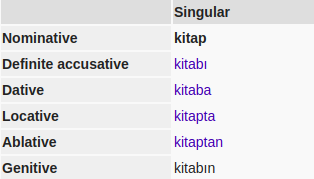
\includegraphics[width=8cm]{images/Turkish_kitap.png}
\centering
\caption{Nominal declension in Turkish, an Oghuz Turkic language (Wiktionary).}
\end{figure}

\begin{figure}[ht]
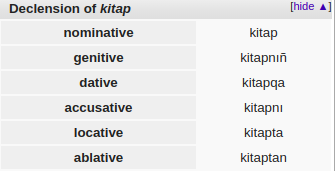
\includegraphics[width=8cm]{images/Crimean_Tatar_kitap.png}
\centering
\caption{Nominal declension in Crimean Tatar, a Kipchak Turkic language (Wiktionary).}
\end{figure}

\begin{figure}[p]
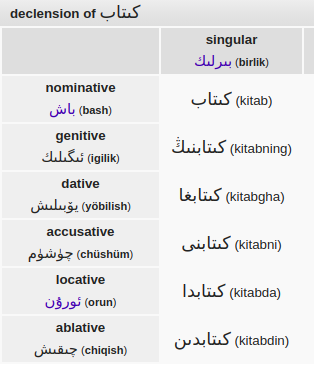
\includegraphics[width=8cm]{images/Uyghur_kitap.png}
\centering
\caption{Nominal declension in Uyghur, a Karluk Turkic language (Wiktionary).}
\end{figure}

For instance, the above declension tables for the word \textit{kitap} "book" show that three languages from different primary branches of the Turkic family all share the same set of noun cases, with cognate suffixes.

Contrast this with inflection of the respective words for "book" in Swedish and Czech, two Indo-European languages of different subfamilies.

\begin{figure}[p]

\includegraphics[width=13cm]{images/Swedish_bok.png}
\centering
\caption{Nominal declension in Swedish, a Germanic Indo-European language (Wiktionary).}
\end{figure}

\begin{figure}[p]
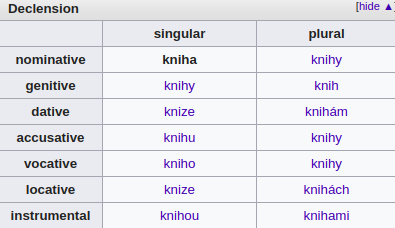
\includegraphics[width=8cm]{images/Czech_kniha.png}
\centering
\caption{Nominal declension in Czech, a Slavic Indo-European language (Wiktionary).}
\end{figure}

\newpage

Given that removing closely related languages from consideration was necessary to generate any statistically significant results, if Turkic languages are designated as "Distantly related" while being quite similar, this might obscure otherwise significant results. And indeed, that seems to have occurred in at least one place: a statistically significant (p<.05) relationship emerges between genealogical distance and model performance. If all language pairs with Turkic target languages are removed from the data set, and genealogical distance is mapped onto a continuous space from 0 (different language family) to 1 (different subfamilies of the same language family) to 2 (same family and subfamily), the previously non-significant negative relationship between genealogical closeness and model performance appears to be statistically confirmed. This result implies that transferred knowledge about a genealogically related source language actually somehow hinders or confuses a model of a target language, contrary to the conclusions of \cite{McCarthy2019}.

\begin{figure}[ht]
\includegraphics[width=12cm]{images/generated/significant/Accuracy_Improvement_vs_2018_vs_Genealogical_distance_non-Turkic_languages.png}
\centering
\caption{Language pair genealogical similarity has a significant negative relationship with model performance once Turkic languages are removed from the data set.}
\end{figure}

This study does not currently possess systematic evidence that the Turkic language family is less diverse than other included language families. Finding a way to include measures of lexical similarity or otherwise measure language relatedness in a more refined way would allow for much more effective and convincing amelioration of the confounding effect of linguistic genealogical relationships.